\newcommand{\ClassPath}{../VIU_TFM_LaTeX_template}
\documentclass{\ClassPath/viu-tfm-template}
\usepackage{multicol}

\definecolor{maincolor}{HTML}{f25416}

%--------------------------------------------------------------------------
% Definiciones necesarias Modifica con tus datos
%--------------------------------------------------------------------------
\def\nombre{ Gómez Olivencia, Rubén}
\def\dni{78910013-A}
\def\titulo{Gestor de contraseñas y documentación \linebreak\linebreak sensible en entorno multiusuario \linebreak\linebreak hecho con Angular y Hashicorp Vault}
\def\subtitulo{(Trabajo Fin de Máster)}
\def\titulacion{Máster Universitario en Desarrollo de Aplicaciones y Servicios Web}
\def\curso{2022-2023 (Ed. Abril)}

%Los siguientes son opcionales: si no se ponen, la portada cambia un poco. Ideal para escribir artículos/trabajos cortos
\def\dirige{Simarro Moncholí, Héctor}
\def\codirige{de Fez Lava, Ismael}
\def\convocatoria{Primera}
\def\asignatura{}


% importar fichero de Bibliografía
\addbibresource{tfm.bib}

\begin{document}
\graphicspath{{../VIU_TFM_LaTeX_template/}}

\coverpage


%--------------------------------------------------------------------------
% Abstract
%--------------------------------------------------------------------------

% Creo un “abstract” propio, porque la plantilla “book” no la tiene, y cambiar a “report” no aporta nada nuevo. Aparte, el comando “abstract” original hace salto de página.

\vspace*{\fill}
\begin{center}
    \textbf{Resumen}
\end{center}

La gestión de contraseñas y documentación que una empresa acumula puede llegar a resultar un problema si no se sabe gestionar de manera correcta. Esta documentación puede crecer si es una empresa de servicios informáticos, con varios clientes, distintos proyectos, contraseñas para distintos servicios...

Existen distintas herramientas que están especializadas en gestión de contraseñas o para gestión de documentación, lo que requeriría tener dos aplicaciones distintas. Muchas veces es conveniente tener la documentación de lo realizado junto con la contraseña de acceso, para así poder facilitar la gestión.

Aparte, estas aplicaciones pueden ser de pago, no tendremos la certeza de cómo es la seguridad real de los datos, ya que normalmente la información no está en nuestros servidores y pueden existir fallos de seguridad que expongan nuestros datos. También hay que tener en cuenta que pueden no ajustarse a nuestras necesidades y salvo que sea una aplicación de Software Libre, no podremos realizar modificaciones

Este TFM trata de aproximar la creación de un gestor de contraseñas y documentación sensible creado en Angular y haciendo uso de Hashicorp Vault como almacenamiento seguro.

\keywords{gestión de contraseñas, seguridad, autenticación, autorización, documentación sensible, cifrado de datos, hashicorp vault}

\vspace*{\fill}
\vspace*{\fill}
\vspace*{\fill}

\pagebreak

%--------------------------------------------------------------------------
% end of Abstract
%--------------------------------------------------------------------------


\tableofcontents


\chapter{Introducción}
En la era digital en la que nos encontramos guardar datos e información es relativamente sencillo, gracias a que cada vez conseguimos tener discos duros con mayor capacidad. En caso de que un único disco duro se nos quede pequeño, existen sistemas como RAID que nos permite combinar varios discos añadiendo tolerancia a fallos en caso de rotura de alguno de ellos.

Por otro lado, tenemos información sensible como son las contraseñas, que a pesar de ocupar poco espacio, debemos tener especial cuidado con ellas, ya que no deben ser accedidas ni utilizadas por personas que no sean su responsabilidad.

En el ámbito personal existen distintas posibilidades que nos permiten gestionar las contraseñas, ya sea de manera integrada en los navegadores web, o a través de aplicaciones externas.

Cuando esta gestión de contraseñas se pasa al ámbito empresarial, a pesar de que también existen distintas alternativas, puede que no cuenten con características necesarias para la empresa; quizá la integración con los sistemas de la empresa no sea posible; en caso de ser una opción de pago ser demasiado cara... Puede resultar complejo decantarse por una solución existente.

A las contraseñas también hay que añadir la información sensible que maneja la empresa, ya sea información propia o de terceras empresas (clientes o proveedores que se tengan). Esa información, ya no tiene por qué ceñirse a “usuario” y “contraseña”, si no que puede ser documentación, ficheros, imágenes, esquemas de red ...

Encontrar una aplicación que se ciña a todas las necesidades puede resultar complejo, y más si estas necesidades varían a lo largo del tiempo. También pueden surgir distintos problemas: la aplicación que utilicemos puede ser abandonada por los creadores; si es de pago, el precio o la suscripción puede variar; la posibilidad de añadir características propias no será posible salvo que sea Software Libre, ...

A lo largo de este \textbf{trabajo final del Máster Universitario en Desarrollo de Aplicaciones y Servicios Web} se analizará la creación de un sistema gestor de contraseñas y documentación sensible para entornos multiusuarios, hecho con el \textit{frontend} de desarrollo \href{https://angular.io/}{Angular} y utilizando  \href{https://www.vaultproject.io/}{Hashicorp Vault} como sistema de backend.


\chapter{Objetivos}
%TODO: añadir introducción
El objetivo principal de este proyecto final de máster es el de aunar los conocimientos adquiridos en el máster y utilizarlos para llevar a cabo una investigación sobre el uso y las funcionalidades de los gestores de contraseñas más conocidos.

Tras este análisis se realizará la propuesta para la realización de un gestor de contraseñas, con los objetivos marcados para el mismo, y cómo se ha realizado su implementación.

\chapter{Estado del arte}

Para acotar el análisis, vamos a identificar qué se entiende por un gestor de contraseñas. ... %TODO:


\section{Gestores de contraseñas conocidos}


\subsection{Problemas acontecidos}



\chapter{Requisitos del proyecto}
Como propuesta para la creación de un gestor de contraseñas propio, se han identificado los siguientes requisitos que deben de cumplirse para considerar que el trabajo final de máster ha cumpido con su objetivo principal:

\begin{itemize}

    \item Se quiere crear un sistema que \textbf{gestione contraseñas e información sensible}. Esta información sensible puede ser imágenes, documentos, o ficheros en general que la aplicación permitirá subir.

    También se podrá generar documentación en la propia aplicación a través de un interfaz \textbf{WYSIWYG} (\textit{what you see is what you get}) que guarde la información en formato Markdown.

    \item El sistema estará basado en web creado con el \textit{framework frontend} \href{https://angular.io/}{Angular} tratando que sea lo más modular posible.

    \item El gestor de contraseñas debe contar con un \textbf{sistema de autenticación}. Sólo debe permitir el acceso a las personas que hayan pasado algún sistema de verificación que demuestre ser quién es.

    Este sistema de autenticación no tiene por qué limitarse al clásico “usuario y contraseña”, si no que podrá adaptarse para utilizar otros sistemas conocidos de forma sencilla, como por ejemplo: certificados \textbf{TLS}, contraseñas de un sólo uso basadas en tiempo (TOTP), tokens basados en \href{https://en.wikipedia.org/wiki/JSON_Web_Token}{JWT}, sistemas \href{https://en.wikipedia.org/wiki/OAuth}{OAuth}/\href{https://en.wikipedia.org/wiki/OpenID#OpenID_Connect_(OIDC)}{OIDC}, ...

    \item Debe existir un \textbf{sistema de autorización, que controle el tipo de acceso y permisos} que tenga en en cuenta quién los realiza y a qué contraseñas se quiere acceder.

    Estos permisos pueden basarse en \textbf{roles}, para de esta manera poder agrupar usuarios, y en base a ellos facilitar la autorización

    \item Para tener un registro de lo sucedido, también es importante contar con un \textbf{sistema de auditoría}. A través de él se registrarán los accesos y operaciones que se realizan.

    \item Lógicamente, la \textbf{seguridad en el acceso y en el almacenamiento} debe ser la principal prioridad. \textbf{Hay que evitar cualquier tipo de acceso a los datos}, ya sea a través del almacenamiento, o por la transmisión de los datos, \textbf{no sea mediante algún sistema  cifrado}.

    De esta manera, en caso de que la información sea interceptada, al estar cifrada, carecerá de sentido y no se podrá visualizar el contenido.



    \item La aplicación debe ser \textbf{sencilla de utilizar}, para que al usuario final no le cueste utilizarla. De esta manera \textbf{conseguiremos que el usuario final la integre en su metodología de trabajo} a la hora de crear/usar contraseñas y guardar información sensible.

    \item Es importante que la aplicación \textbf{se adapte a la pantalla} donde se esté visualizando. De esta manera el usuario podrá hacer uso de ella a través de dispositivos móviles.

    \item Para el almacenamiento de la información y el sistema de autorización se hará uso del sistema \href{https://www.vaultproject.io/}{Vault} de la empresa \href{https://www.hashicorp.com/}{Hashicorp}.
\end{itemize}

Teniendo en cuenta las metodologías utilizadas, y explicadas en el siguiente apartado, cualquier añadido a estos requisitos se podría añadir en etapas posteriores del desarrollo.


\chapter{Metodologías utilizadas}

Hoy en día es conveniente hacer uso de las \textbf{metodologías ágiles} cuando realizamos la gestión de un proyecto, ya que cuentan con una serie de ventajas que nos van a permitir dar una respuesta más rápida y flexible ante posibles cambios durante la vida de desarrollo del producto.

Ventajas que podemos destacar de las metodologías ágiles:

\begin{itemize}
    \item Poder entregar resultados funcionales al cliente cada poco tiempo y así obtener \textit{feedback} de lo realizado.
    \item Seremos capaces de dar una respuesta ágil y flexible ante posibles cambios que puedan surgir (cambios en los requisitos, ante bajas de personal asignado al proyecto, dificultades durante el desarrollo...).
    \item Tratar de evitar burocracia innecesaria, para centrarnos de esta manera en el producto y sus funcionalidades.
    \item Se trata de involucrar al cliente y colaborar con él para de esta manera conseguir un mayor valor al producto.
\end{itemize}

\section{Gestión del proyecto}

Para comenzar con la gestión del proyecto debemos contar con los objetivos nombrados previamente y transformarlos en las conocidas como “\textbf{historias de usuario}”.

En ellas plasmaremos, en un lenguaje que pueda entender el cliente, las funcionalidades que el producto debe tener, a las que asociaremos otros datos como son:

\begin{itemize}
    \item Un \textbf{identificador único} para poder diferenciarlas del resto.
    \item Una \textbf{estimación de tiempos} de lo que creemos que podemos tardar en realizarlo.
    \item La \textbf{prioridad} inicial para poder ordenarlas entre ellas.
    \item El \textbf{tema principal} al que se relaciona la historia de usuario.
    \item Se añadirán posibles \textbf{dependencias} de otras historias de usuario.
    \item Una \textbf{descripción} de lo que se quiere conseguir.
    \item Unos \textbf{criterios de validación} por parte del cliente.
\end{itemize}

\subsection{Resultado del análisis realizado}

A continuación se van a plasmar las distintas “historias de usuario” obtenidas:

\begin{requisitostbl}{X[1]X[2]X[2]X[3]X[2]}
    ID & Estimación & Prioridad  & Tema &  Dependencias \\
    1  & 25 horas & 1  & Interfaz web &   \\

    Desarrollar “esqueleto” del interfaz web \\

    \textbf{Descripción}:
    Como usuario necesito un interfaz web para poder acceder a la aplicación y hacer uso de ella. Es la base del proyecto. \\

    \textbf{Criterios de validación}:
    El interfaz es \textit{\textbf{responsive}}, visualmente atractivo y funcional. \\
\end{requisitostbl}

\begin{requisitostbl}{X[1]X[2]X[2]X[3]X[2]}
    ID & Estimación & Prioridad  & Tema &  Dependencias \\
    2  & 10 horas & 1  & Gestión de usuarios & 1  \\

    Crear “login” de usuario \\

    \textbf{Descripción}:
    Como usuario quiero poder acceder a la aplicación utilizando como sistema de autenticación un usuario y contraseña.  \\

    \textbf{Criterios de validación}:
    Los valores introducidos serán autenticados contra el \textit{backend} que el cliente decida (base de datos o LDAP/Active Directory). \\
\end{requisitostbl}

\begin{requisitostbl}{X[1]X[2]X[2]X[3]X[2]}
    ID & Estimación & Prioridad  & Tema &  Dependencias \\
    3  & 10 horas & 1  & Gestión de Secretos & 2  \\

    Crear secretos \\

    \textbf{Descripción}:
    Como usuario quiero poder crear un secreto para poder guardar información sensible y/o contraseñas. \\

    \textbf{Criterios de validación}:
    \begin{itemize}
        \item El botón para crear siempre será visible.
        \item Se podrá elegir la ruta (por defecto será donde nos encontramos) y el nombre del secreto.
    \end{itemize}
    \\
\end{requisitostbl}



\begin{requisitostbl}{X[1]X[2]X[2]X[3]X[2]}
    ID & Estimación & Prioridad  & Tema &  Dependencias \\
    4  & 30 horas & 1  & Gestión de Secretos & 2, 3  \\

    Listado de secretos \\

    \textbf{Descripción}:
    Como usuario quiero poder obtener un listado de los secretos existentes para poder navegar por ellos y seleccionar el que me interese. \\

    \textbf{Criterios de validación}:
    \begin{itemize}
        \item El listado completo se visualiza mediante un árbol jerarquizado.
        \item También se puede navegar como si fuera un explorador de archivos.
        \item El interfaz mostrará un \textit{breadcrumb} para indicar la ruta en la que nos encontramos.
        \item Se puede buscar por el nombre de los secretos.
    \end{itemize}
    \\
\end{requisitostbl}



\begin{requisitostbl}{X[1]X[2]X[2]X[3]X[2]}
    ID & Estimación & Prioridad  & Tema &  Dependencias \\
    5  & 15 horas & 2  & Gestión de Secretos & 2, 3, 4  \\

    Visualizar un secreto \\

    \textbf{Descripción}:
    Como usuario quiero acceder a un secreto para visualizar su contenido.  \\

    \textbf{Criterios de validación}:
    \begin{itemize}
        \item La visualización mostrará el secreto en formato HTML.
        \item Si un usuario accede a un secreto “bloqueado” el sistema lo debe alertar y no se le permitirá editarlo.
        \item El interfaz nos mostrará la última vez que se modificó el secreto.
        \item Al visualizar el secreto aparecerán botones con distintas acciones que se podrán realizar sobre él (editar, imprimir, ver históricos, borrar).
    \end{itemize}
    \\
\end{requisitostbl}


\begin{requisitostbl}{X[1]X[2]X[2]X[3]X[2]}
    ID & Estimación & Prioridad  & Tema &  Dependencias \\
    6  & 35 horas & 2  & Gestión de Secretos & 2, 3  \\

    Modificar un secreto \\

    \textbf{Descripción}:
    Como usuario quiero poder editar un secreto para realizar modificaciones.  \\

    \textbf{Criterios de validación}:
    \begin{itemize}
        \item La modificación se realizará a través de un editor \textit{\textbf{WYSIWYG}}.
        \item El editor permitirá realizar modificaciones en formato \href{https://es.wikipedia.org/wiki/Markdown}{Markdown}.
        \item El editor permitirá guardar el secreto y al hacerlo volveremos a la visualización del mismo.
        \item Al comenzar la modificación el secreto se pondrá en estado “bloqueado”.
    \end{itemize}
    \\
\end{requisitostbl}



\begin{requisitostbl}{X[1]X[2]X[2]X[3]X[2]}
    ID & Estimación & Prioridad  & Tema &  Dependencias \\
    7  & 10 horas & 3  & Gestión de Secretos & 2, 3, 5  \\

    Borrado de secretos \\

    \textbf{Descripción}:
    Como usuario quiero poder borrar secretos para que desaparezcan.  \\

    \textbf{Criterios de validación}:
    \begin{itemize}
        \item Antes de borrar debe existir un mensaje de confirmación.
        \item Al borrar un secreto, el árbol de secretos se debe actualizar.
    \end{itemize}
     \\
\end{requisitostbl}



\begin{requisitostbl}{X[1]X[2]X[2]X[3]X[2]}
    ID & Estimación & Prioridad  & Tema &  Dependencias \\
    8  & 15 horas & 3  & Gestión de Secretos & 2  \\

    Permitir gestionar ficheros como secretos \\

    \textbf{Descripción}:
    Como usuario quiero poder subir ficheros al sistema para guardarlos cifrados.  \\

    \textbf{Criterios de validación}:
    \begin{itemize}
        \item Se permite subir cualquier tipo de fichero.
        \item Se permite descargar el fichero original.
        \item Se debe poder visualizar los ficheros más habituales en la propia web (imágenes y ficheros PDF) sin necesidad de descargarlos.
    \end{itemize}
     \\
\end{requisitostbl}


\begin{requisitostbl}{X[1]X[2]X[2]X[3]X[2]}
    ID & Estimación & Prioridad  & Tema &  Dependencias \\
    9  & 20 horas & 4  & Gestión de Secretos & 3, 6  \\

    Versionado de secretos\\

    \textbf{Descripción}:
    Como usuario quiero poder ver las veces que el fichero ha sido modificado para poder ver los cambios realizados.  \\

    \textbf{Criterios de validación}:
    \begin{itemize}
        \item Poder ver el número de versiones que tiene un secreto.
        \item Poder ver una versión concreta del secreto.
        \item Poder ver las diferencias entre versiones.
        \item Poder restaurar una versión concreta del secreto.
    \end{itemize} \\
\end{requisitostbl}


\begin{requisitostbl}{X[1]X[2]X[2]X[3]X[2]}
    ID & Estimación & Prioridad  & Tema &  Dependencias \\
    10  & 5 horas & 4  & Gestión de Secretos & 2, 5  \\

    Imprimir secretos \\

    \textbf{Descripción}:
    Como usuario quiero poder imprimir un secreto. \\

    \textbf{Criterios de validación}:
    Existe un botón para imprimir un secreto. \\
\end{requisitostbl}



\begin{requisitostbl}{X[1]X[2]X[2]X[3]X[2]}
    ID & Estimación & Prioridad  & Tema &  Dependencias \\
    11  & 35 horas & 2  & Producción & 1  \\

    Puesta en producción segura \\

    \textbf{Descripción}:
    Como usuario quiero poder acceder a la plataforma de manera segura para realizar todo lo comentado hasta ahora \\

    \textbf{Criterios de validación}:
    \begin{itemize}
        \item El acceso web tiene que ser por HTTPS (certificado válido).
        \item El servidor debe estar securizado ante accesos externos.
        \item Los servicios deben auto-arrancarse en caso de caída.
        \item Existe un registro de lo sucedido a cada secreto (auditoría).
    \end{itemize} \\
\end{requisitostbl}


\subsection{Mapa de las historias de usuario}

Dado que las historias de usuario pueden suponer la agrupación de distintas tareas técnicas que son más pequeñas, es conveniente crear un mapa que englobe todas las tareas a realizar.

Para la organización de este mapa se pueden identificar los siguientes apartados:
\begin{itemize}
    \item Los \textbf{temas} son las características a alto nivel que va a tener la aplicación, y coinciden con el tema de las historias de usuario. En el mapa se ha diferenciado en color verde.
    \item Los \textbf{epics}, en color azul, son características que normalmente no pueden realizarse en un \textit{sprint}, que a veces pueden ser divididas en distintas historias de usuarios, y que engloban en su mayoría varias tareas.
    \item Las \textbf{tareas}, en este caso en amarillo, son las unidades concretas de trabajo. Se ha tratado que sean lo más cortas posibles y que a nivel técnico sean auto-contenidas y aisladas.
\end{itemize}

El mapa resultante inicial para la gestión del proyecto es el siguiente:

\begin{center}
    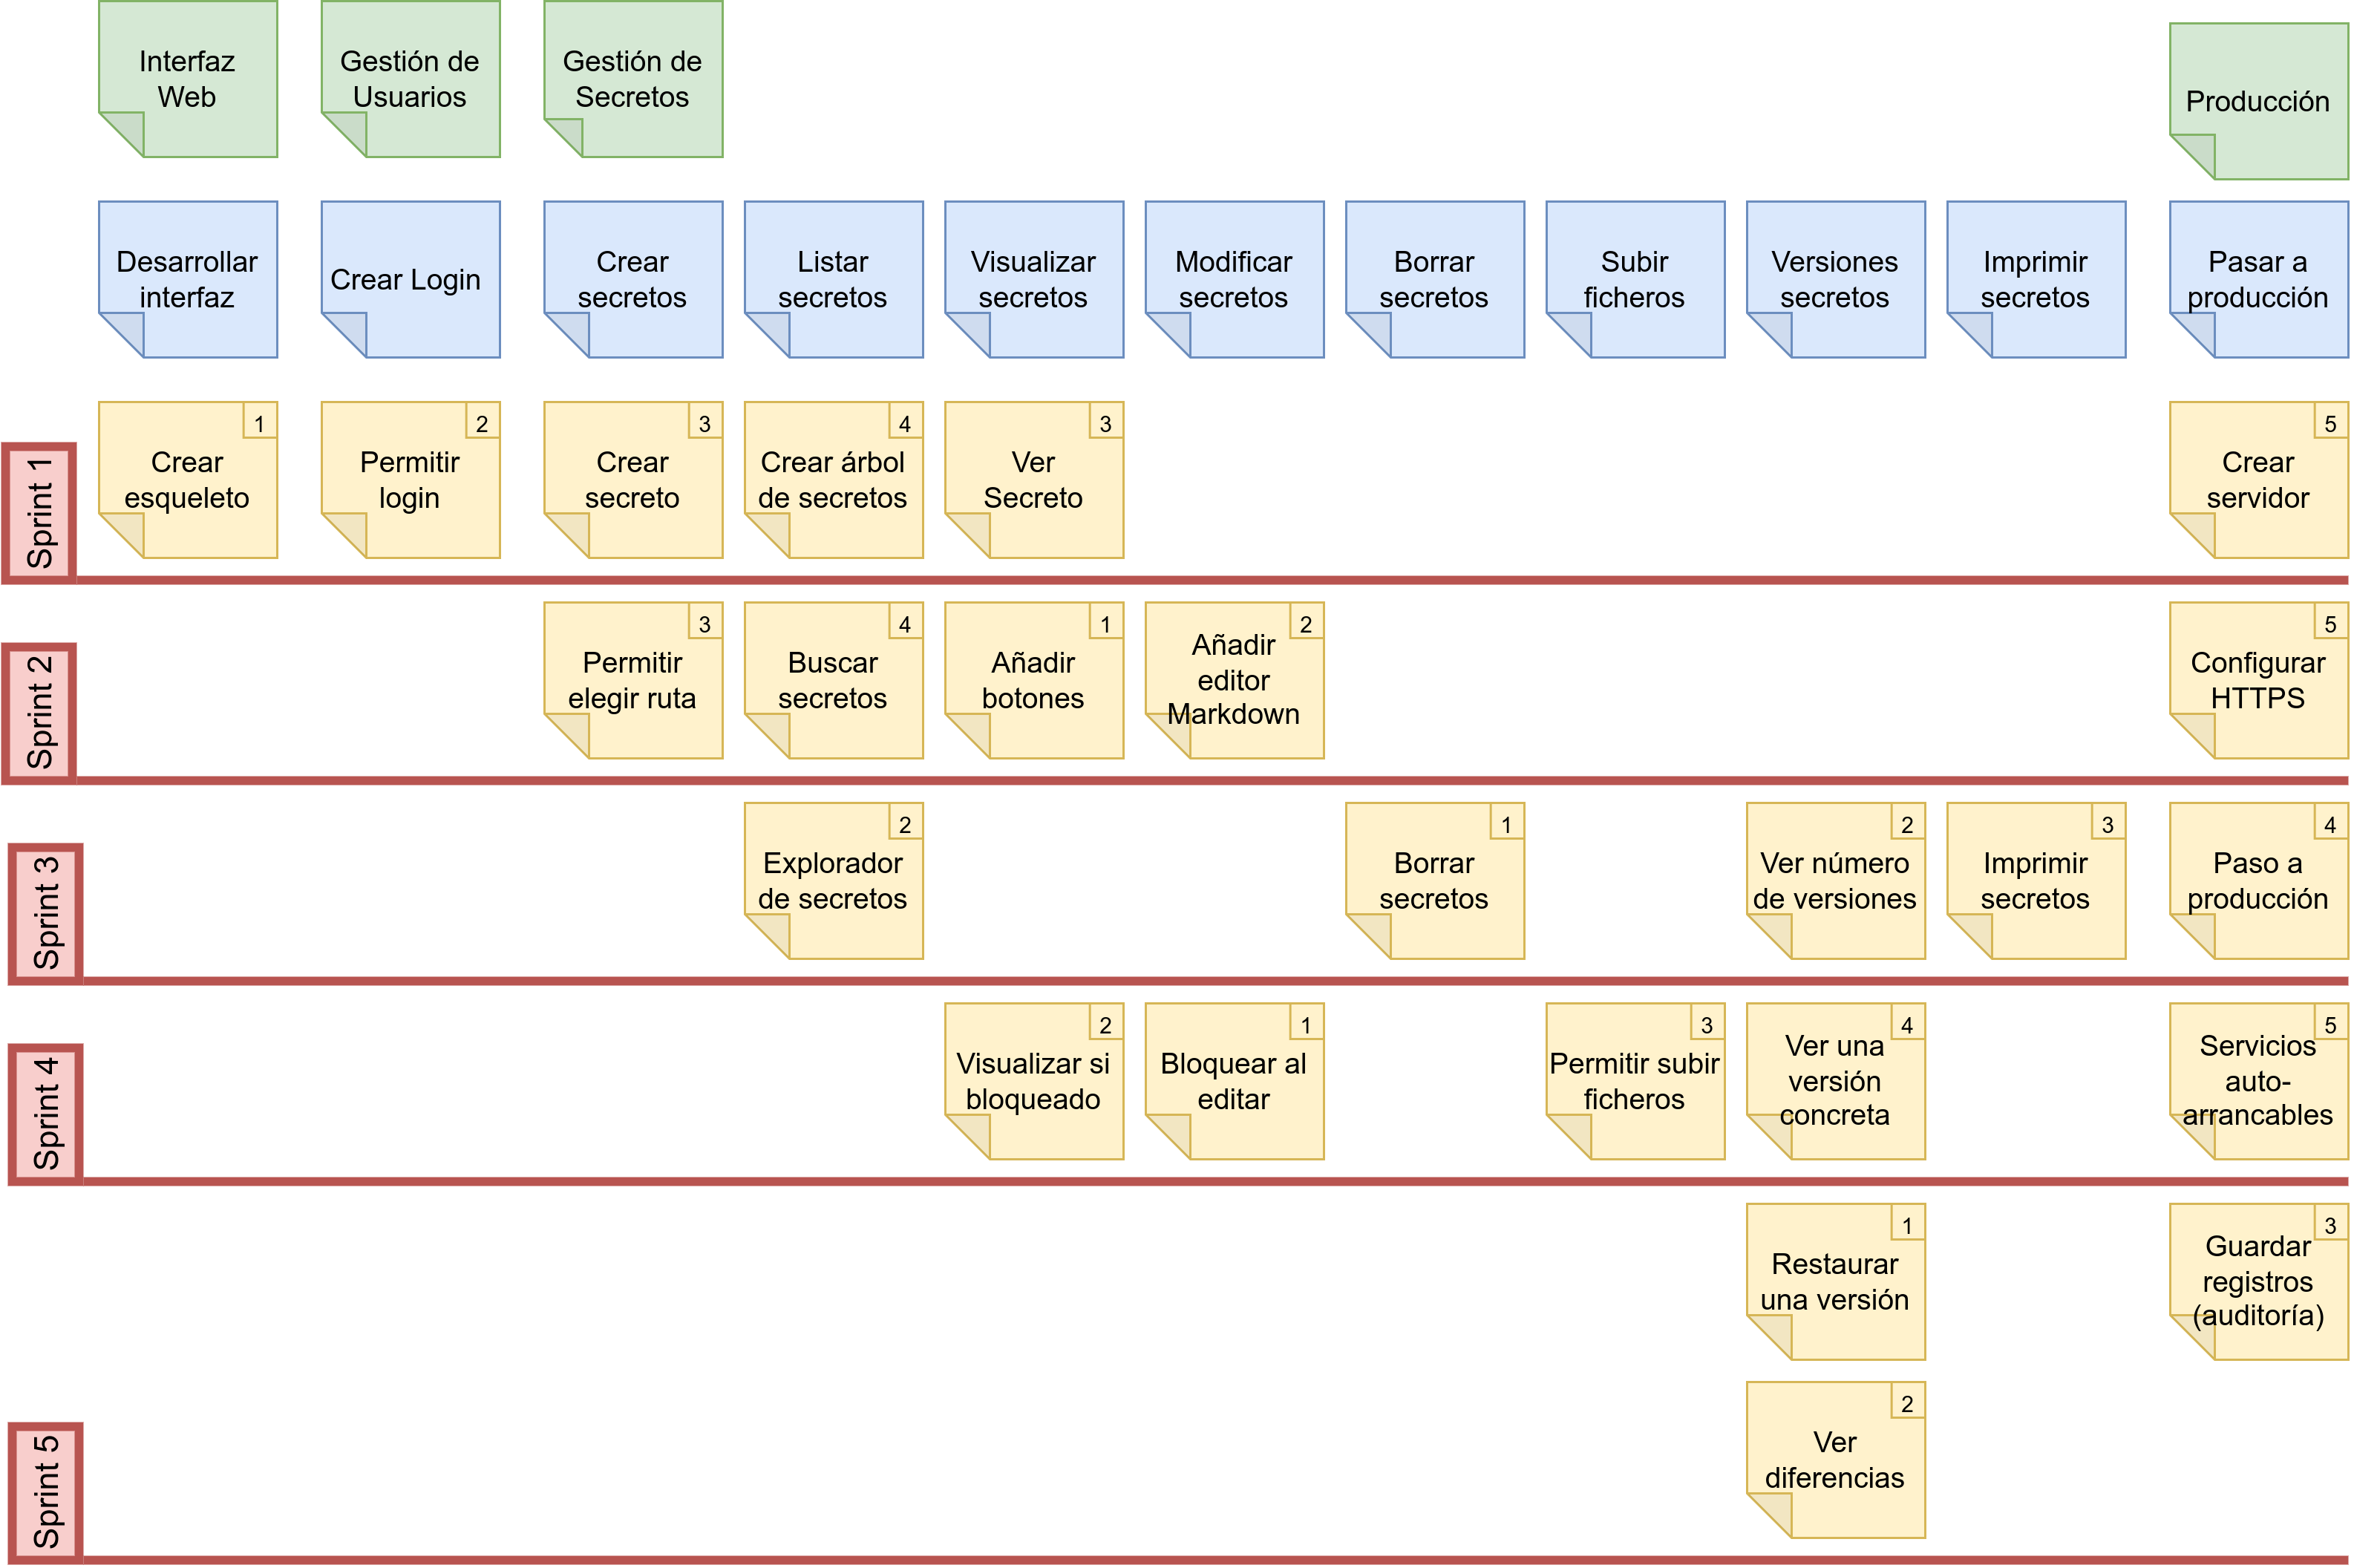
\includegraphics[width=\linewidth]{img/kanban.png}
\end{center}

\subsection{\textit{Sprints} generados}

A la par que se ha ido creando el mapa anterior, se han diferenciado diferentes \textit{sprints} con las tareas que deberían completarse para cada uno de ellos.

Bien es cierto que aunque haya sido realizada esa primera estimación, se podrían efectuar modificaciones en caso de que fuese necesario.

Para el primer \textit{sprint} se han identificado las siguientes tareas que deben realizarse:

\begin{center}
    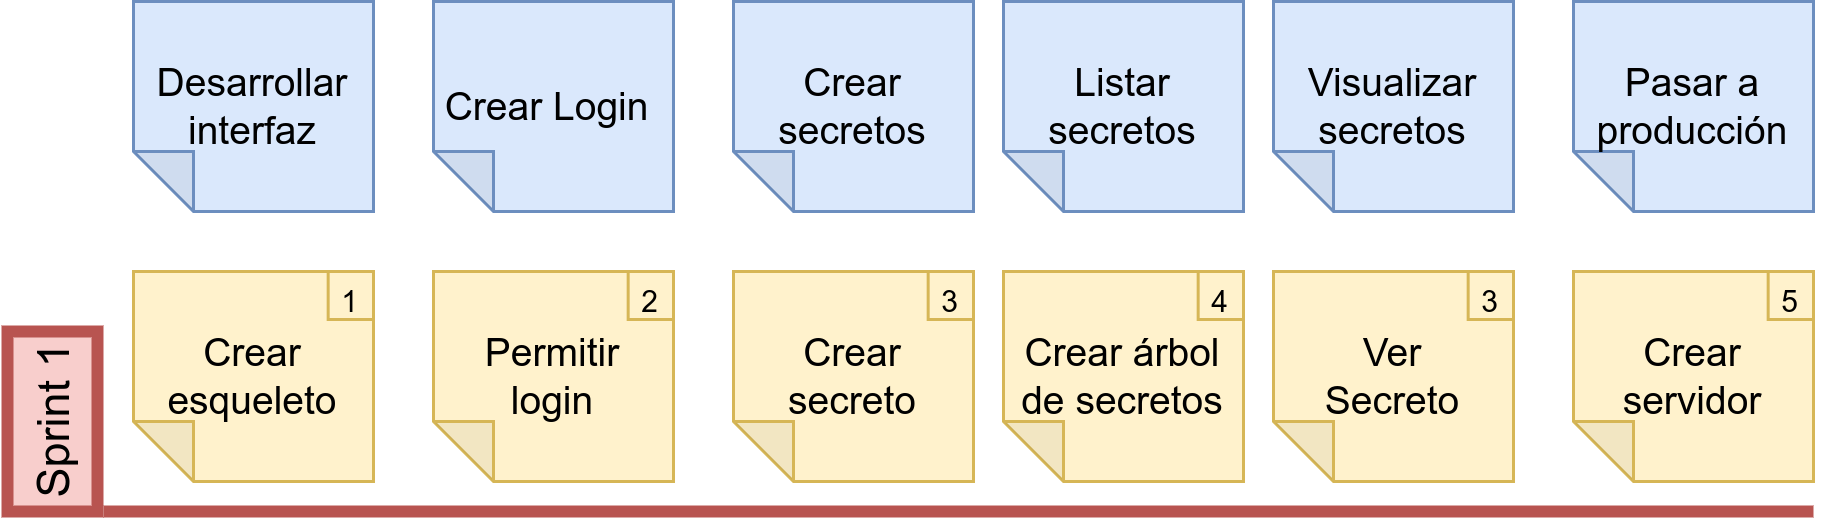
\includegraphics[width=\linewidth]{img/sprint1.png}
\end{center}

Tal como se puede ver, las tareas están representadas con su prioridad dentro del \textit{sprint}, para así también tener claro qué tareas deben tratar de terminarse antes que otras.

Al terminar este primer \textit{sprint}, tendremos la base del proyecto terminada, y podríamos mostrarle al cliente una primera versión con unas funcionalidades básicas.

De esta manera, podemos obtener \textit{feedback} de lo realizado, con una base ya terminada. Ese \textit{feedback} podremos utilizarlo como retroalimentación para el siguiente \textit{sprint}, ya sea para realizar modificaciones de lo ya realizado (hacer cambios nuevos que el cliente pida) o para utilizarlo para las tareas ya planificadas.



\section{Herramientas tecnológicas utilizadas}

Durante la implementación del proyecto hemos hecho uso de distintas herramientas tecnológicas, que a su vez también nos han ayudado con las metodologías ágiles explicadas previamente:

\subsection{Gestión de tareas en Trello}

\href{https://trello.com/}{Trello} es una aplicación web, creada por la empresa \href{https://www.atlassian.com/}{Atlassian}, que nos permite tener un tablero \href{https://en.wikipedia.org/wiki/Kanban_(development)}{Kanban} donde podremos añadir las tareas de nuestro proyecto, e ir moviéndolas entre distintas etapas.

Aunque cuenta con una versión de suscripción, la versión gratuita cuenta con las características suficientes como para poder ser utilizado para la gestión de proyectos sin problema alguno.

Una vez definidas las tareas, tal como se ha visto anteriormente, se han añadido a Trello, en el que se han creado las siguientes columnas, o fases de desarrollo:

\begin{itemize}
    \item \textbf{Tareas pendientes}: donde situaremos las tareas que se deben realizar para llevar a cabo el proyecto.

\end{itemize}

\begin{minipage}{0.6\linewidth}
    \begin{itemize}
        \item \textbf{Desarrollo}: Son las tareas que se han empezado a desarrollar.
        \item \textbf{Testing}: Son las tareas que se dan por terminadas en el desarrollo y que pasan a una fase de testeo. En algunos casos puede ser directamente testeado por el cliente para dar su feedback (por ejemplo para el interfaz web), aunque lo habitual es que el testeo lo realice otra persona del proyecto (que no haya sido quien ha hecho el desarrollo).

        En caso de que una tarea no pase esta fase, se anotará los inconvenientes y volverá a la columna de \textbf{desarrollo}.
        \item \textbf{Producción}: Una vez el \textit{testing} ha terminado, se puede dar por terminada la tarea y debe ser incluida en producción.
    \end{itemize}

Tal como se puede ver en la imagen, cada tarea se representa como una pequeña tarjeta, apareciendo como un listado de todas ellas en la columna correspondiente en las que están situadas (en este caso todavía en la tarea de pendientes).
\end{minipage}
\hfill
\begin{minipage}{0.32\linewidth}
        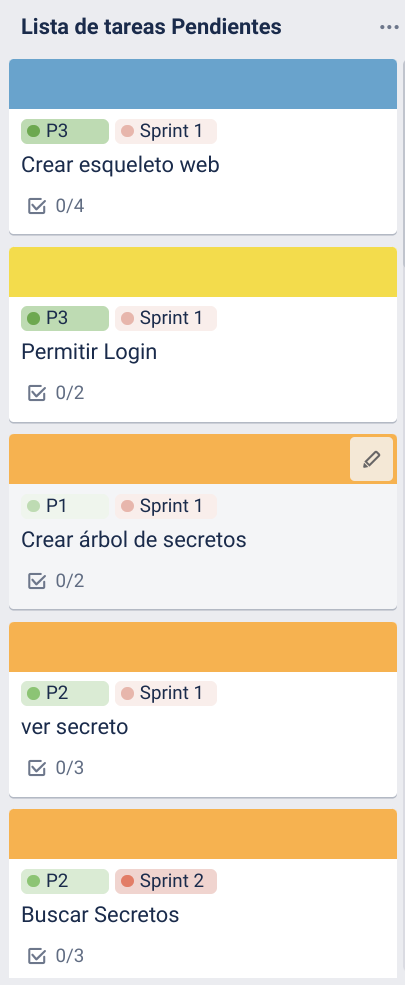
\includegraphics[width=\linewidth]{img/tareas.png}
    \vspace{-30pt}
    \begin{center}
        {\scriptsize \textit{Tareas pendientes en Trello}}
    \end{center}
\end{minipage}

%\vspace{10pt}


A cada una de las tareas se les ha asignado un color teniendo en cuenta el tema al que pertenecen, y varias etiquetas que representan el \textit{sprint} y la prioridad dentro del \textit{sprint}. De esta manera, Trello nos permitirá realizar búsquedas o visualizar las tareas con la etiqueta que nos interese.


\begin{minipage}{0.48\linewidth}
    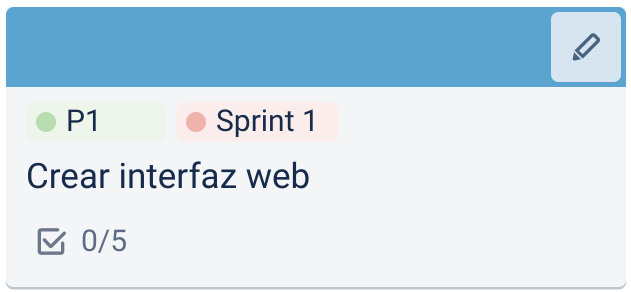
\includegraphics[width=\linewidth]{img/tarea.png}
    \vspace{-30pt}
    \begin{center}
        {\scriptsize \textit{Detalle de tarea}}
    \end{center}
\end{minipage}
\hfill
\begin{minipage}{0.40\linewidth}
    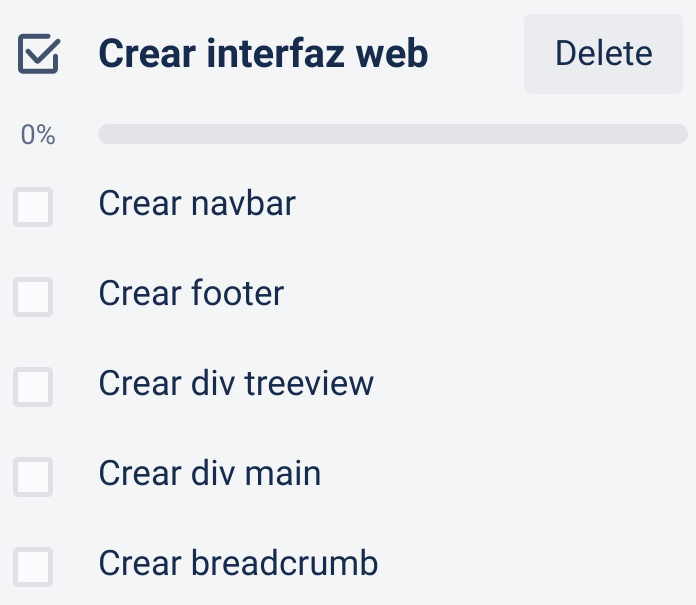
\includegraphics[width=\linewidth]{img/tarea1.png}
    \vspace{-30pt}
    \begin{center}
        {\scriptsize \textit{Ítems de tarea}}
    \end{center}
\end{minipage}

Por último, cada tarea puede tener pequeños ítems. Estos han sido detallados para que a la hora de desarrollar se tenga en cuenta qué es lo que debe conseguir, y de esta manera dar por finalizada la tarea.

Tras terminar la tarea, se pasará a la columna \textbf{testing}, para de esta manera

\subsection{Gestión de código fuente con Git}

\href{https://es.wikipedia.org/wiki/Git}{Git} es el sistema de control de versiones creado por \href{https://es.wikipedia.org/wiki/Linus_Torvalds}{Linus Torvalds} para la gestión del código fuente de \href{https://es.wikipedia.org/wiki/N%C3%BAcleo_Linux}{Linux}. Hoy en día es el sistema más utilizado gracias a características tan importantes como la facilidad para crear ramas, su versatilidad para adaptarse al flujo de trabajo del desarrollador, integración con los entornos de desarrollo más importantes...

A pesar de que Git permite ser descentralizado, se ha utilizado la plataforma \href{https://github.com/}{Github} como plataforma centralizadora y de esta manera también así disponer de una copia de seguridad del código fuente.

\begin{center}
    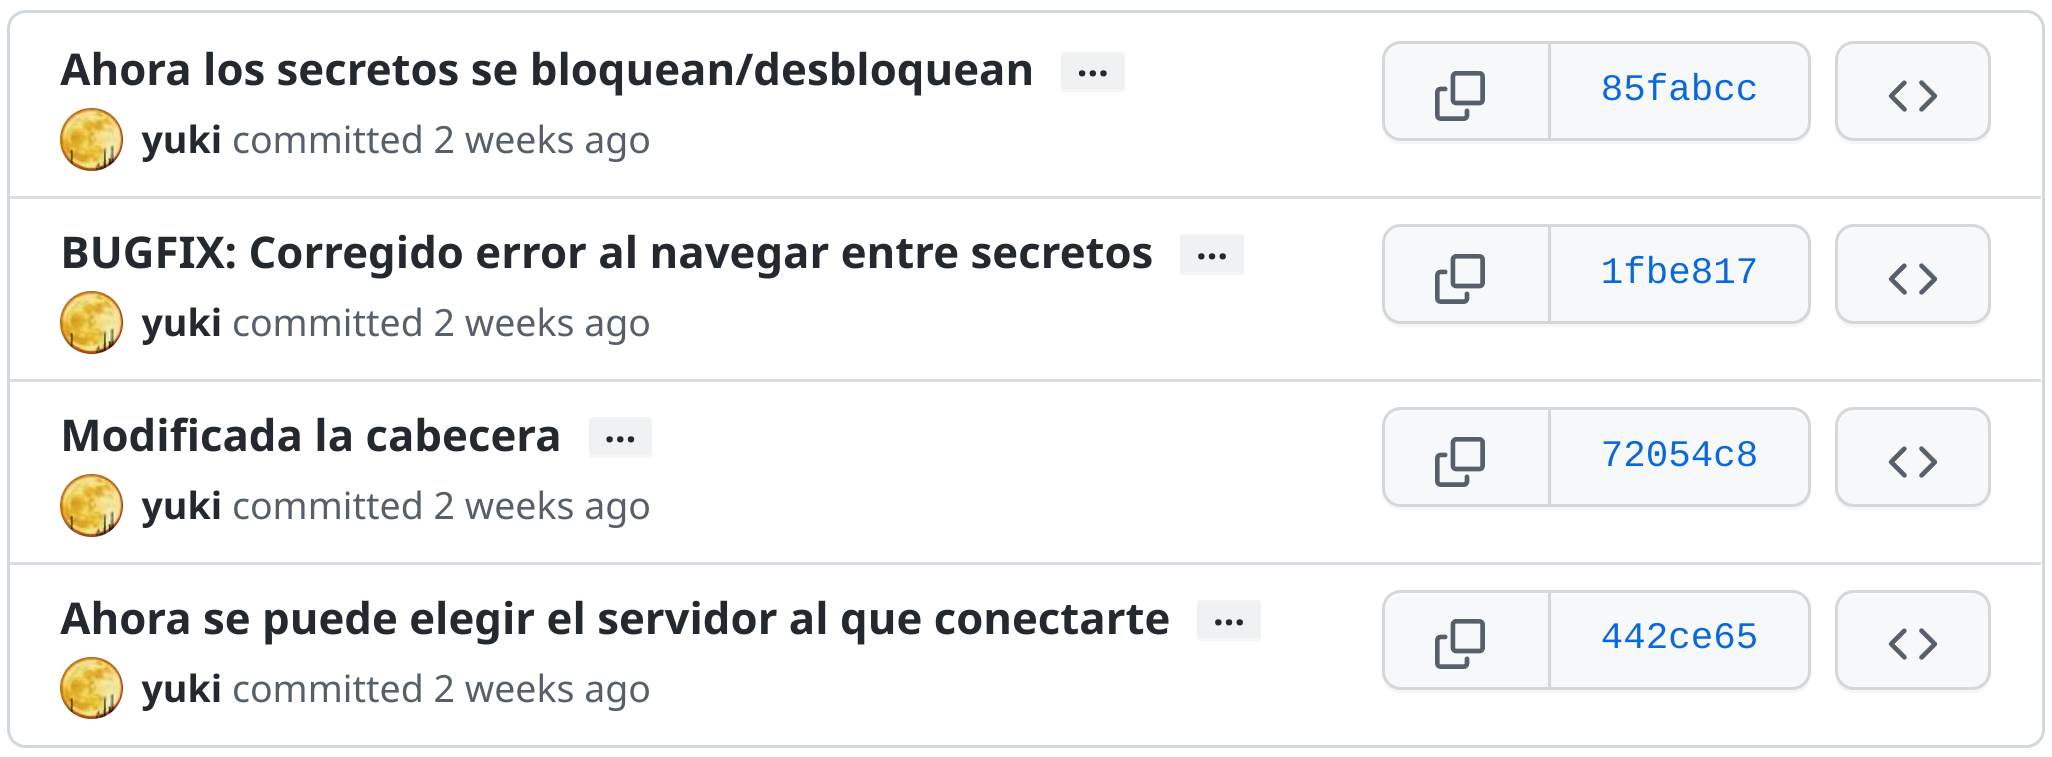
\includegraphics[width=0.8\linewidth]{img/commits.png}
\end{center}

Aparte, también se ha integrado con Trello (a través de los plugins conocidos como “Power-Ups”) para así poder asociar las tareas a los commits que las han cumplimentado. De esta manera conseguiremos una relación “tarea ↔ código” que podremos utilizar para analizar si ha habido algún error durante el desarrollo, o fases como la de \textit{testing}.


\subsection{Creación de entornos con Docker}
Para poder crear distintos entornos aislados para cada una de las fases del desarrollo se ha hecho uso de contenedores \href{https://es.wikipedia.org/wiki/Docker_(software)}{Docker}.




\chapter{Resultados}




\chapter{Trabajo futuro}

% TODO: posibles mejoras a añadir:

% TODO: configuración del usuario, forzar actualizar el árbol, mejor visualización de ficheros, permitir exportar secretos a formatos editables (odt/docx)





\chapter{Conclusiones}



\end{document}
